\documentclass{beamer}
\usepackage[utf8]{inputenc}
\usepackage[T1]{fontenc}
\usepackage[catalan]{babel}
\usepackage{amsmath}
\usepackage{amssymb}
\usepackage{amsthm}
\usepackage{subfigure}

\newtheorem{teorema}{Teorema}
\newtheorem{corollari}{Corol\textperiodcentered lari}
\newtheorem{lema}{Lema}
\newtheorem{definicio}{Definici\'{o}}
\newtheorem{notacio}{Notaci\'{o}}
\newtheorem{proposicio}{Proposici\'{o}}
\newtheorem{observacio}{Observaci\'{o}}
\theoremstyle{definition}
\newtheorem{exemple}{Exemple}

\mode<presentation>
{
\usetheme{Boadilla}
\usecolortheme{seahorse}
}

\DeclareMathOperator{\id}{id}

\title{Espais de moduli}
\author{Alejandro Plaza Gall\'{a}n}
\date{8 de juny de 2021}

\begin{document}

\begin{frame}
\titlepage
\end{frame}

\begin{frame}{Introducci\'{o}}
\begin{itemize}
\item Identifiquem estructures segons relaci\'{o} d'isomorfia.
\pause
\begin{itemize}
\item Conjunts: aplicacions bijectives.
\pause
\item Espais vectorials: isomorfismes d'espais vectorials.
\end{itemize}
\pause
\item Associem invariants a cada classe d'equival\`{e}ncia.
\pause
\begin{itemize}
\item Conjunts: cardinal.
\pause
\item Espais vectorials de dimensi\'{o} finita: dimensi\'{o}.
\end{itemize}
\pause
\item Prenem classes d'equival\`{e}ncia de certes estructures algebraico-geom\`{e}triques i parametritzem les classes d'equival\`{e}ncia.
\end{itemize}
\end{frame}

\begin{frame}{Espai projectiu}
Partim de $\mathbb{R}^2\backslash\{0\}$ i definim la relaci\'{o} d'equival\`{e}ncia tal que per tots $x,y\in\mathbb{R}^2\backslash\{0\}$
\[x\sim y\Leftrightarrow\exists\lambda\in\mathbb{R}:y=\lambda x.\]
\pause
El quocient \'{e}s el conjunt de rectes que passen per l'origen.
\[S=\{L\backslash\{0\}\,|\,L\text{ \'{e}s subespai vectorial de }\mathbb{R}^2,\dim L=1\}\]
\pause

Volem donar una noci\'{o} de dist\`{a}ncia. Podr\'{i}em prendre simplement la topologia quocient.

Tamb\'{e} podem definir una dist\`{a}ncia
\begin{align*}
d:S\times S&\longrightarrow[0,\infty),\\
([x],[y])&\longmapsto\cos\frac{|\langle x,y\rangle|}{||x||||y||}
\end{align*}
que \'{e}s l'angle que formen dues rectes.
\pause

De fet l'espai projectiu es pot identificar amb $\mathbb{S}^1$.
\end{frame}

\begin{frame}{Tors}
Considerem el pla complex $\mathbb{C}$. Considerem el reticle $\mathbb{Z}+i\mathbb{Z}\subseteq\mathbb{C}$ dins del pla. \'{E}s com $\mathbb{Z}\times\mathbb{Z}$ dins $\mathbb{R}^2$.
\pause

$\mathbb{Z}+i\mathbb{Z}\cong\mathbb{Z}^2$ \'{e}s un grup, que actua per l'addici\'{o} sobre $\mathbb{C}$.
\begin{align*}
(\mathbb{Z}+i\mathbb{Z})\times\mathbb{C}&\longrightarrow\mathbb{C}\\
(n+im,z)&\longmapsto(n+im)+z
\end{align*}
\pause
Tota classe de $\mathbb{C}/(\mathbb{Z}+i\mathbb{Z})$ t\'{e} un representant dins el quadrat $[0,1]+i[0,1]$.
\pause
\begin{figure}[ht!]
\begin{center}
\begin{subfigure}{}
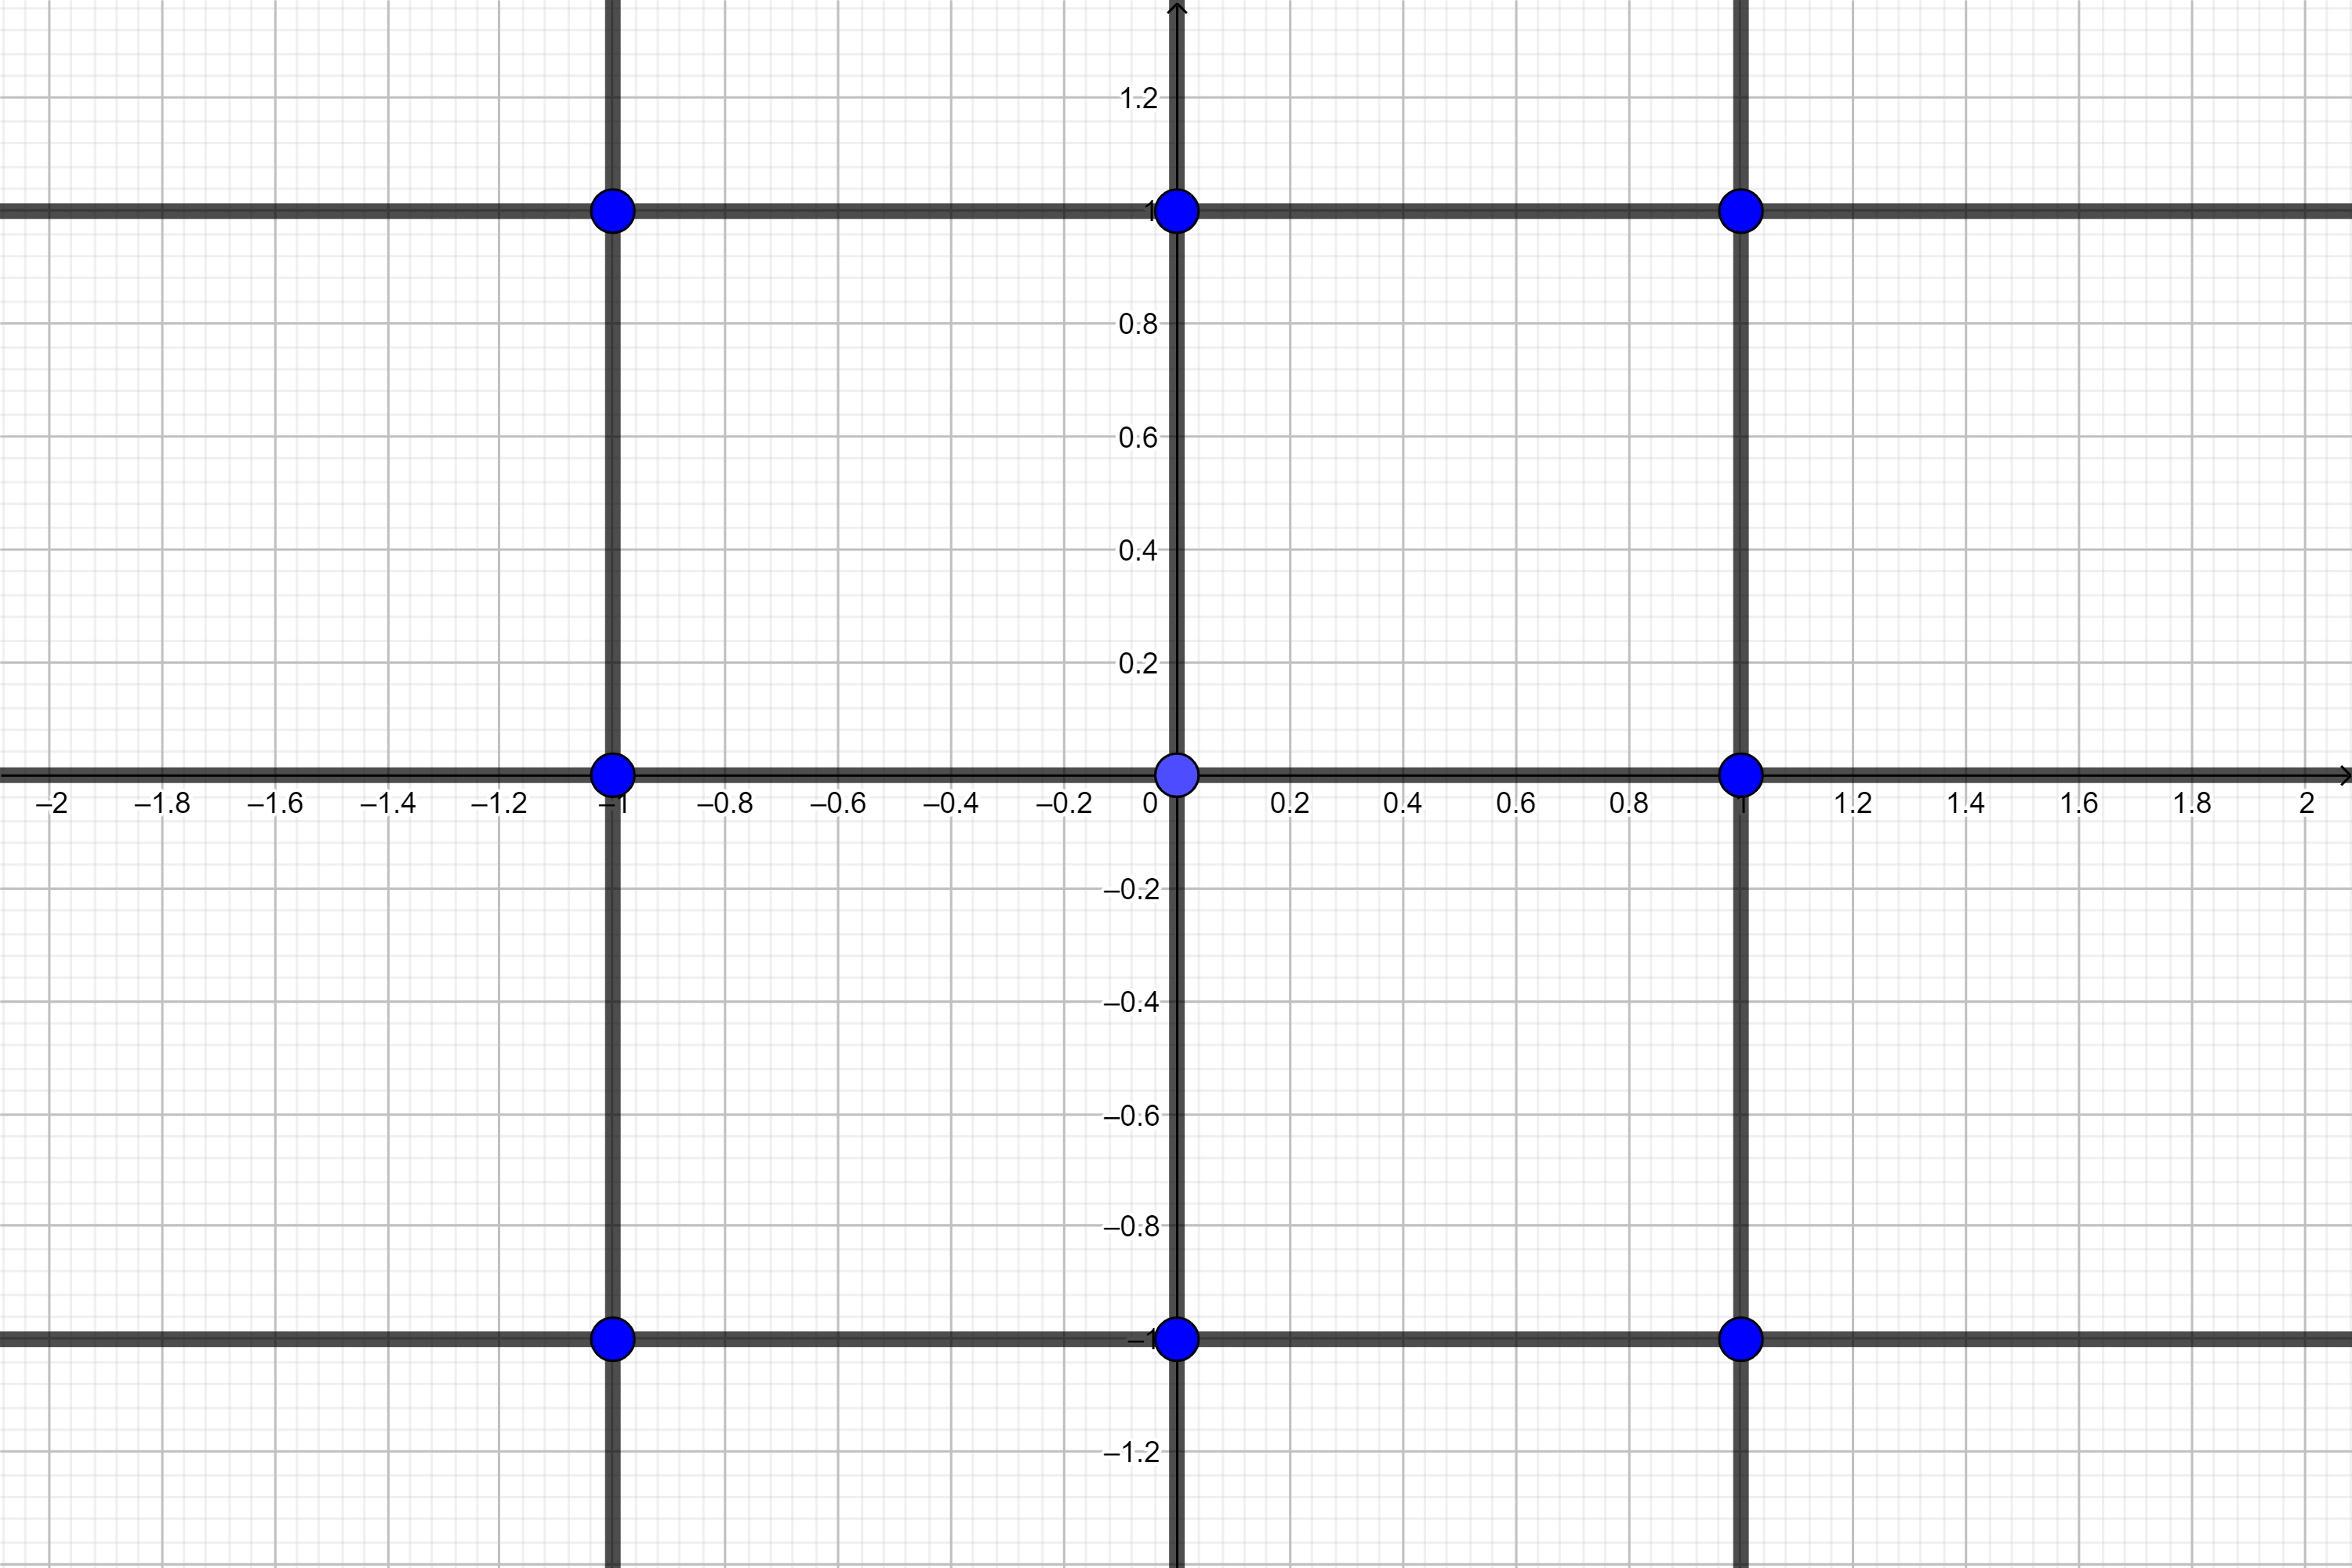
\includegraphics[width=6cm]{Reticlesobri.png} 
\end{subfigure}
\begin{subfigure}{}
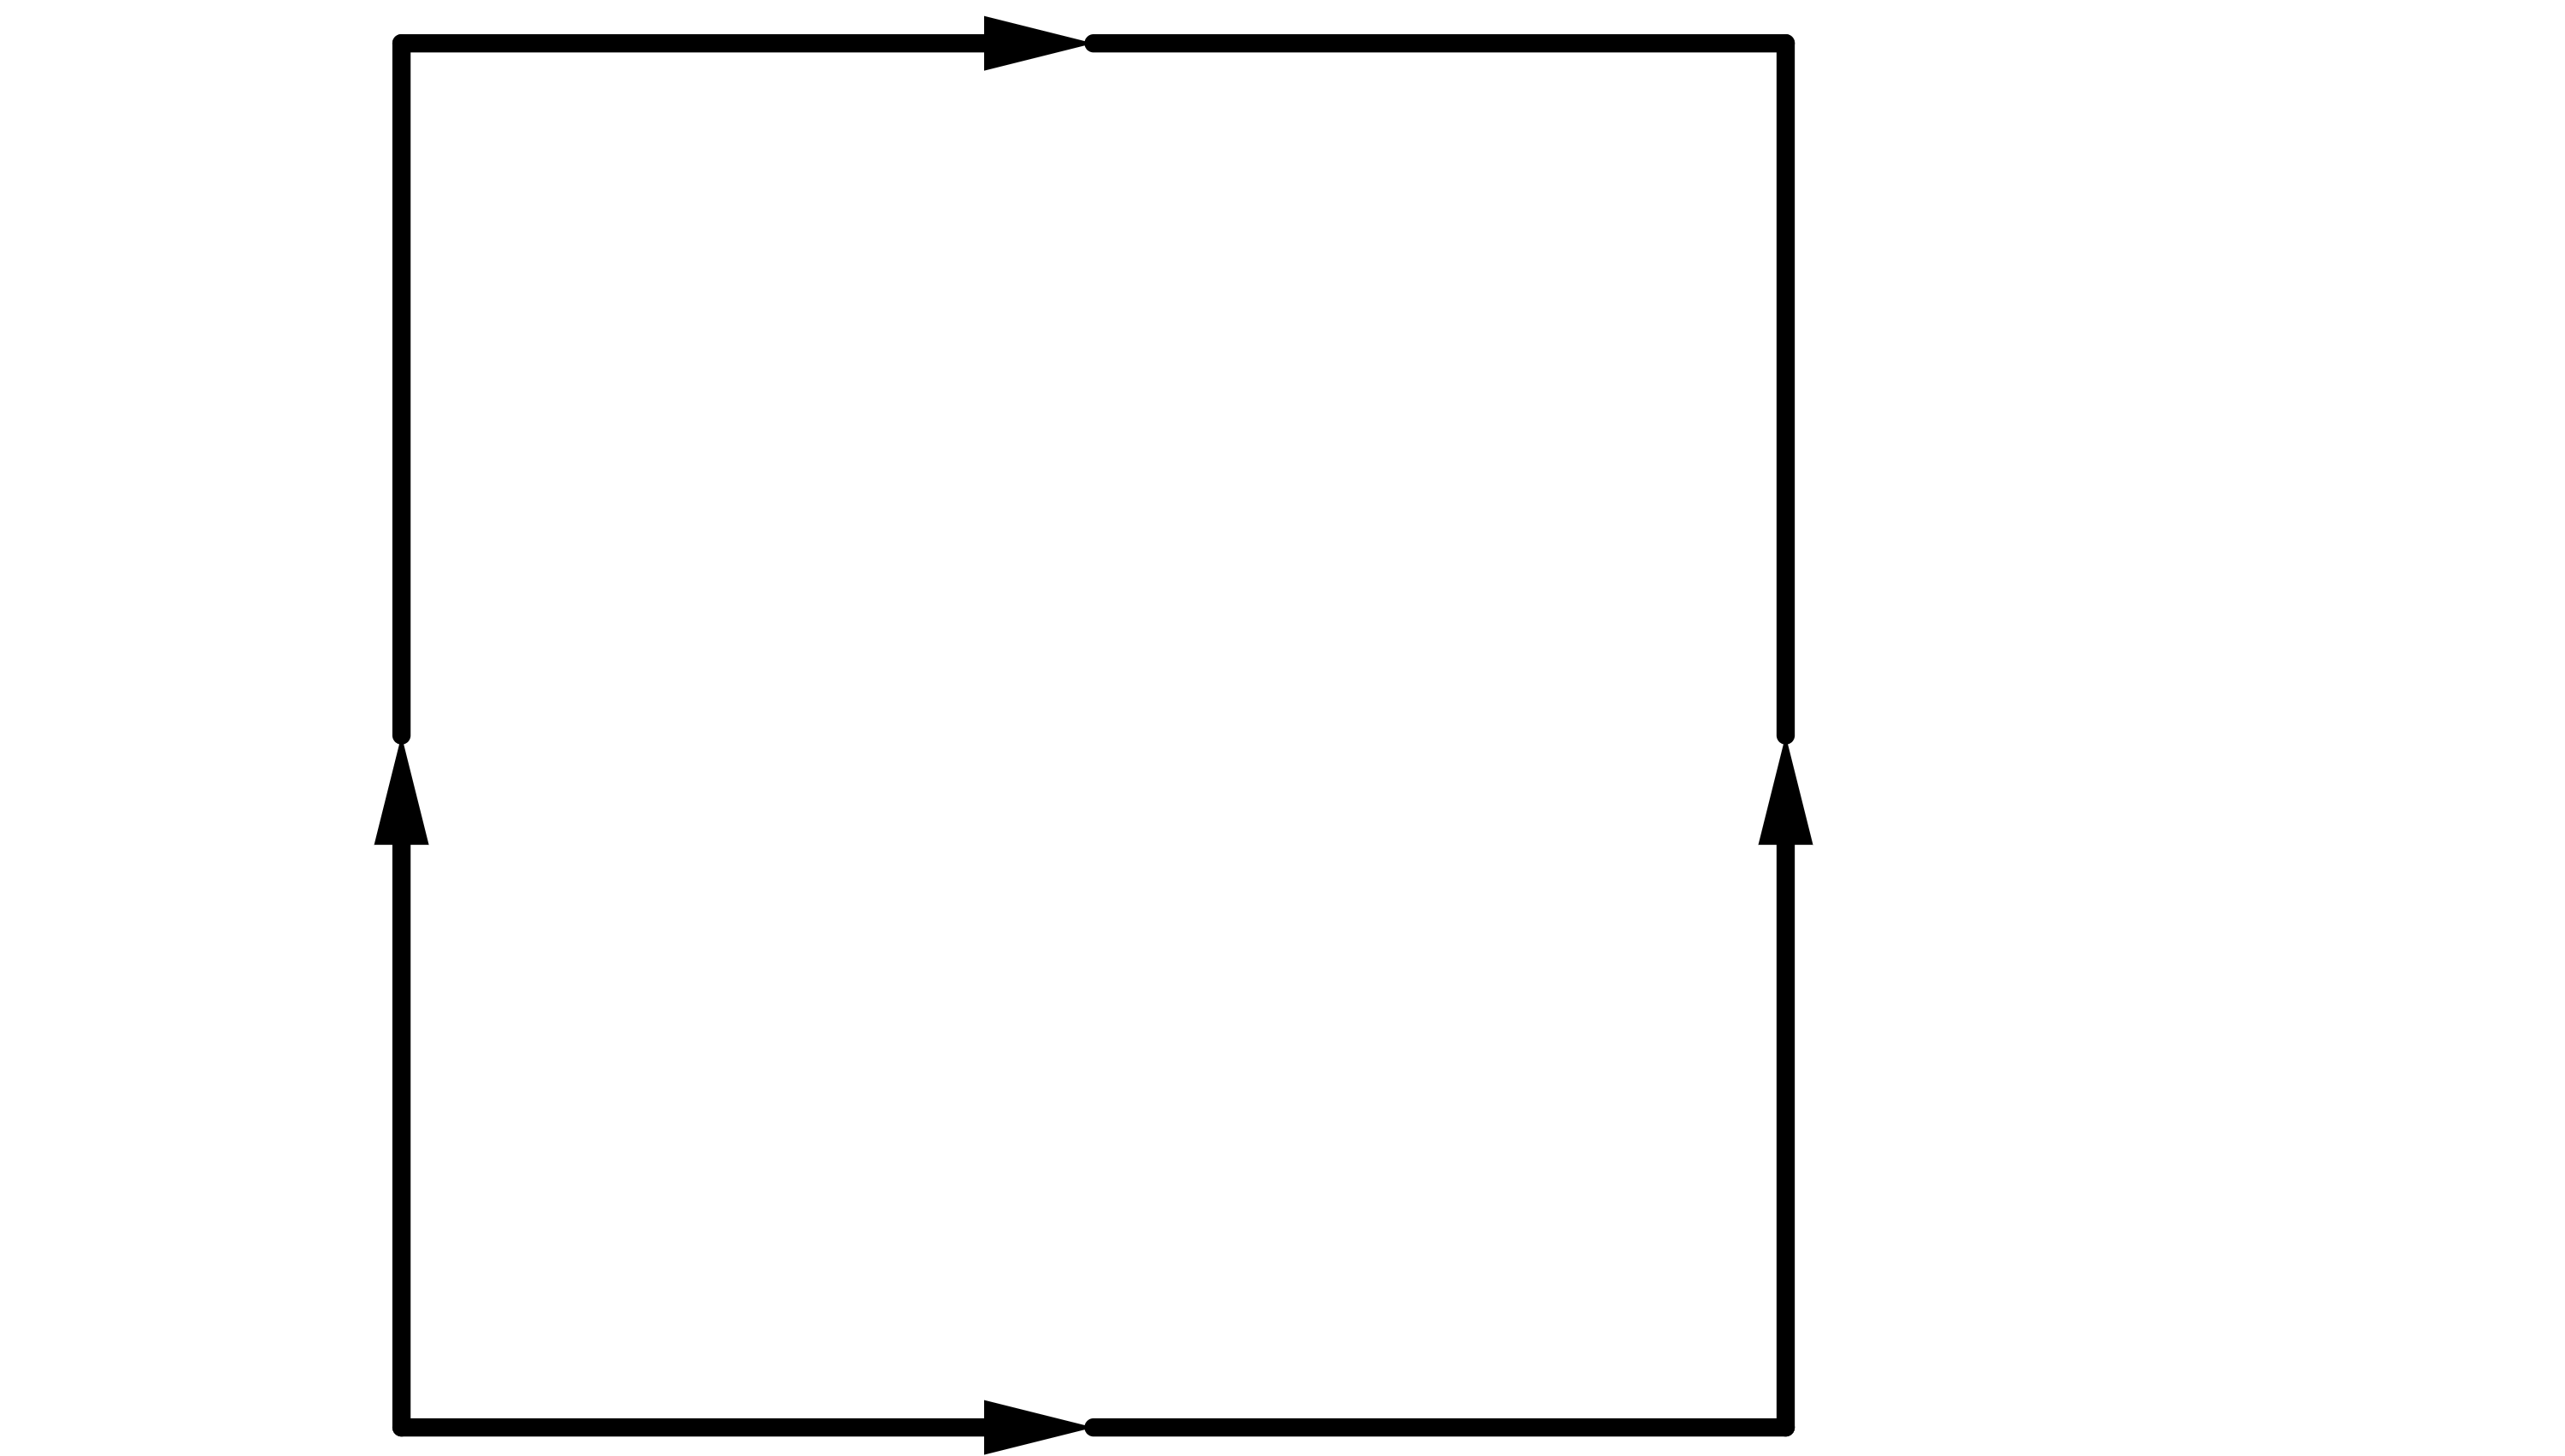
\includegraphics[width=5cm]{Quadratsobri.png} 
\end{subfigure}
\end{center}
\end{figure}
\end{frame}

\begin{frame}{Tors}
\begin{definicio}
Una \textbf{varietat topol\`{o}gica} de dimensi\'{o} $n$ \'{e}s un espai topol\`{o}gic $M$ Hausdorff, segon numerable i localment homeomorf a $\mathbb{R}^n$. Aix\`{o} \'{u}ltim vol dir que per tot $x\in M$ existeixen un entorn obert $U\subseteq M$ de $x$ i un homeomorfisme $\phi:U\rightarrow\mathbb{R}^n$. El parell $(U,\phi)$ es diu \textbf{carta local} de $M$. La inversa d'una carta local es diu \textbf{parametritzaci\'{o}}.
\end{definicio}
\pause
\begin{definicio}
Una \textbf{varietat diferenciable} de dimensi\'{o} $n$ \'{e}s una varietat topol\`{o}gica amb una fam\'{i}lia de cartes locals $\{(U_i,\phi_i)\}_{i\in I}$ anomenada \textbf{atles} que compleix:
\begin{enumerate}
\item $\displaystyle{\bigcup_{i\in I}U_i=M}$
\item $\forall i,j\in I$ el \textbf{canvi de carta} $\phi_j\circ\phi_i^{-1}:\phi_i(U_i\cap U_j)\rightarrow\phi_j(U_i\cap U_j)$ \'{e}s llis. Observem que $\phi_i(U_i\cap U_j),\phi_j(U_i\cap U_j)\subseteq\mathbb{R}^n$.
\end{enumerate}
\end{definicio}
\end{frame}

\begin{frame}{Tors}
\begin{definicio}
Una \textbf{varietat complexa} de dimensi\'{o} $n$ \'{e}s un espai topol\`{o}gic Hausdorff i segon numerable amb un atles $\{(U_i,\phi_i)\}_{i\in I}$ format per cartes locals $\phi_i:U_i\rightarrow\mathbb{C}^n$ que compleixen:
\begin{enumerate}
\item $\displaystyle{\bigcup_{i\in I}U_i=M}$
\item $\forall i,j\in I$, el canvi de carta $\phi_j\circ\phi_i^{-1}:\phi_i(U_i\cap U_j)\rightarrow\phi_j(U_i\cap U_j)$ \'{e}s holomorf. Observem que $\phi_i(U_i\cap U_j),\phi_j(U_i\cap U_j)\subseteq\mathbb{C}^n$.
\end{enumerate}
\end{definicio}
\pause
\begin{definicio}
Un morfisme entre varietats diferenciables o complexes \'{e}s una aplicaci\'{o} $f:M\rightarrow N$ tal que per tota carta local $(U,\phi)$ de $M$ i tota carta local $(V,\psi)$ de $N$, es compleix que $\psi\circ f\circ\phi^{-1}$ \'{e}s diferenciable o holomorfa respectivament.
\end{definicio}
\end{frame}

\begin{frame}{Tors}
\begin{definicio}
Dues varietats diferenciables o complexes s\'{o}n equivalents quan existeix una aplicaci\'{o} $f:M\rightarrow N$ bijectiva amb inversa $f^{-1}:N\rightarrow M$ tal que $f$ i $f^{-1}$ s\'{o}n diferenciables o holomorfes. respectivament.
\end{definicio}
\pause
\begin{definicio}
Una superf\'{i}cie de Riemann \'{e}s una varietat complexa de dimensi\'{o} $1$.
\end{definicio}
\pause
\begin{figure}[ht!]
\begin{center}
\begin{subfigure}{}
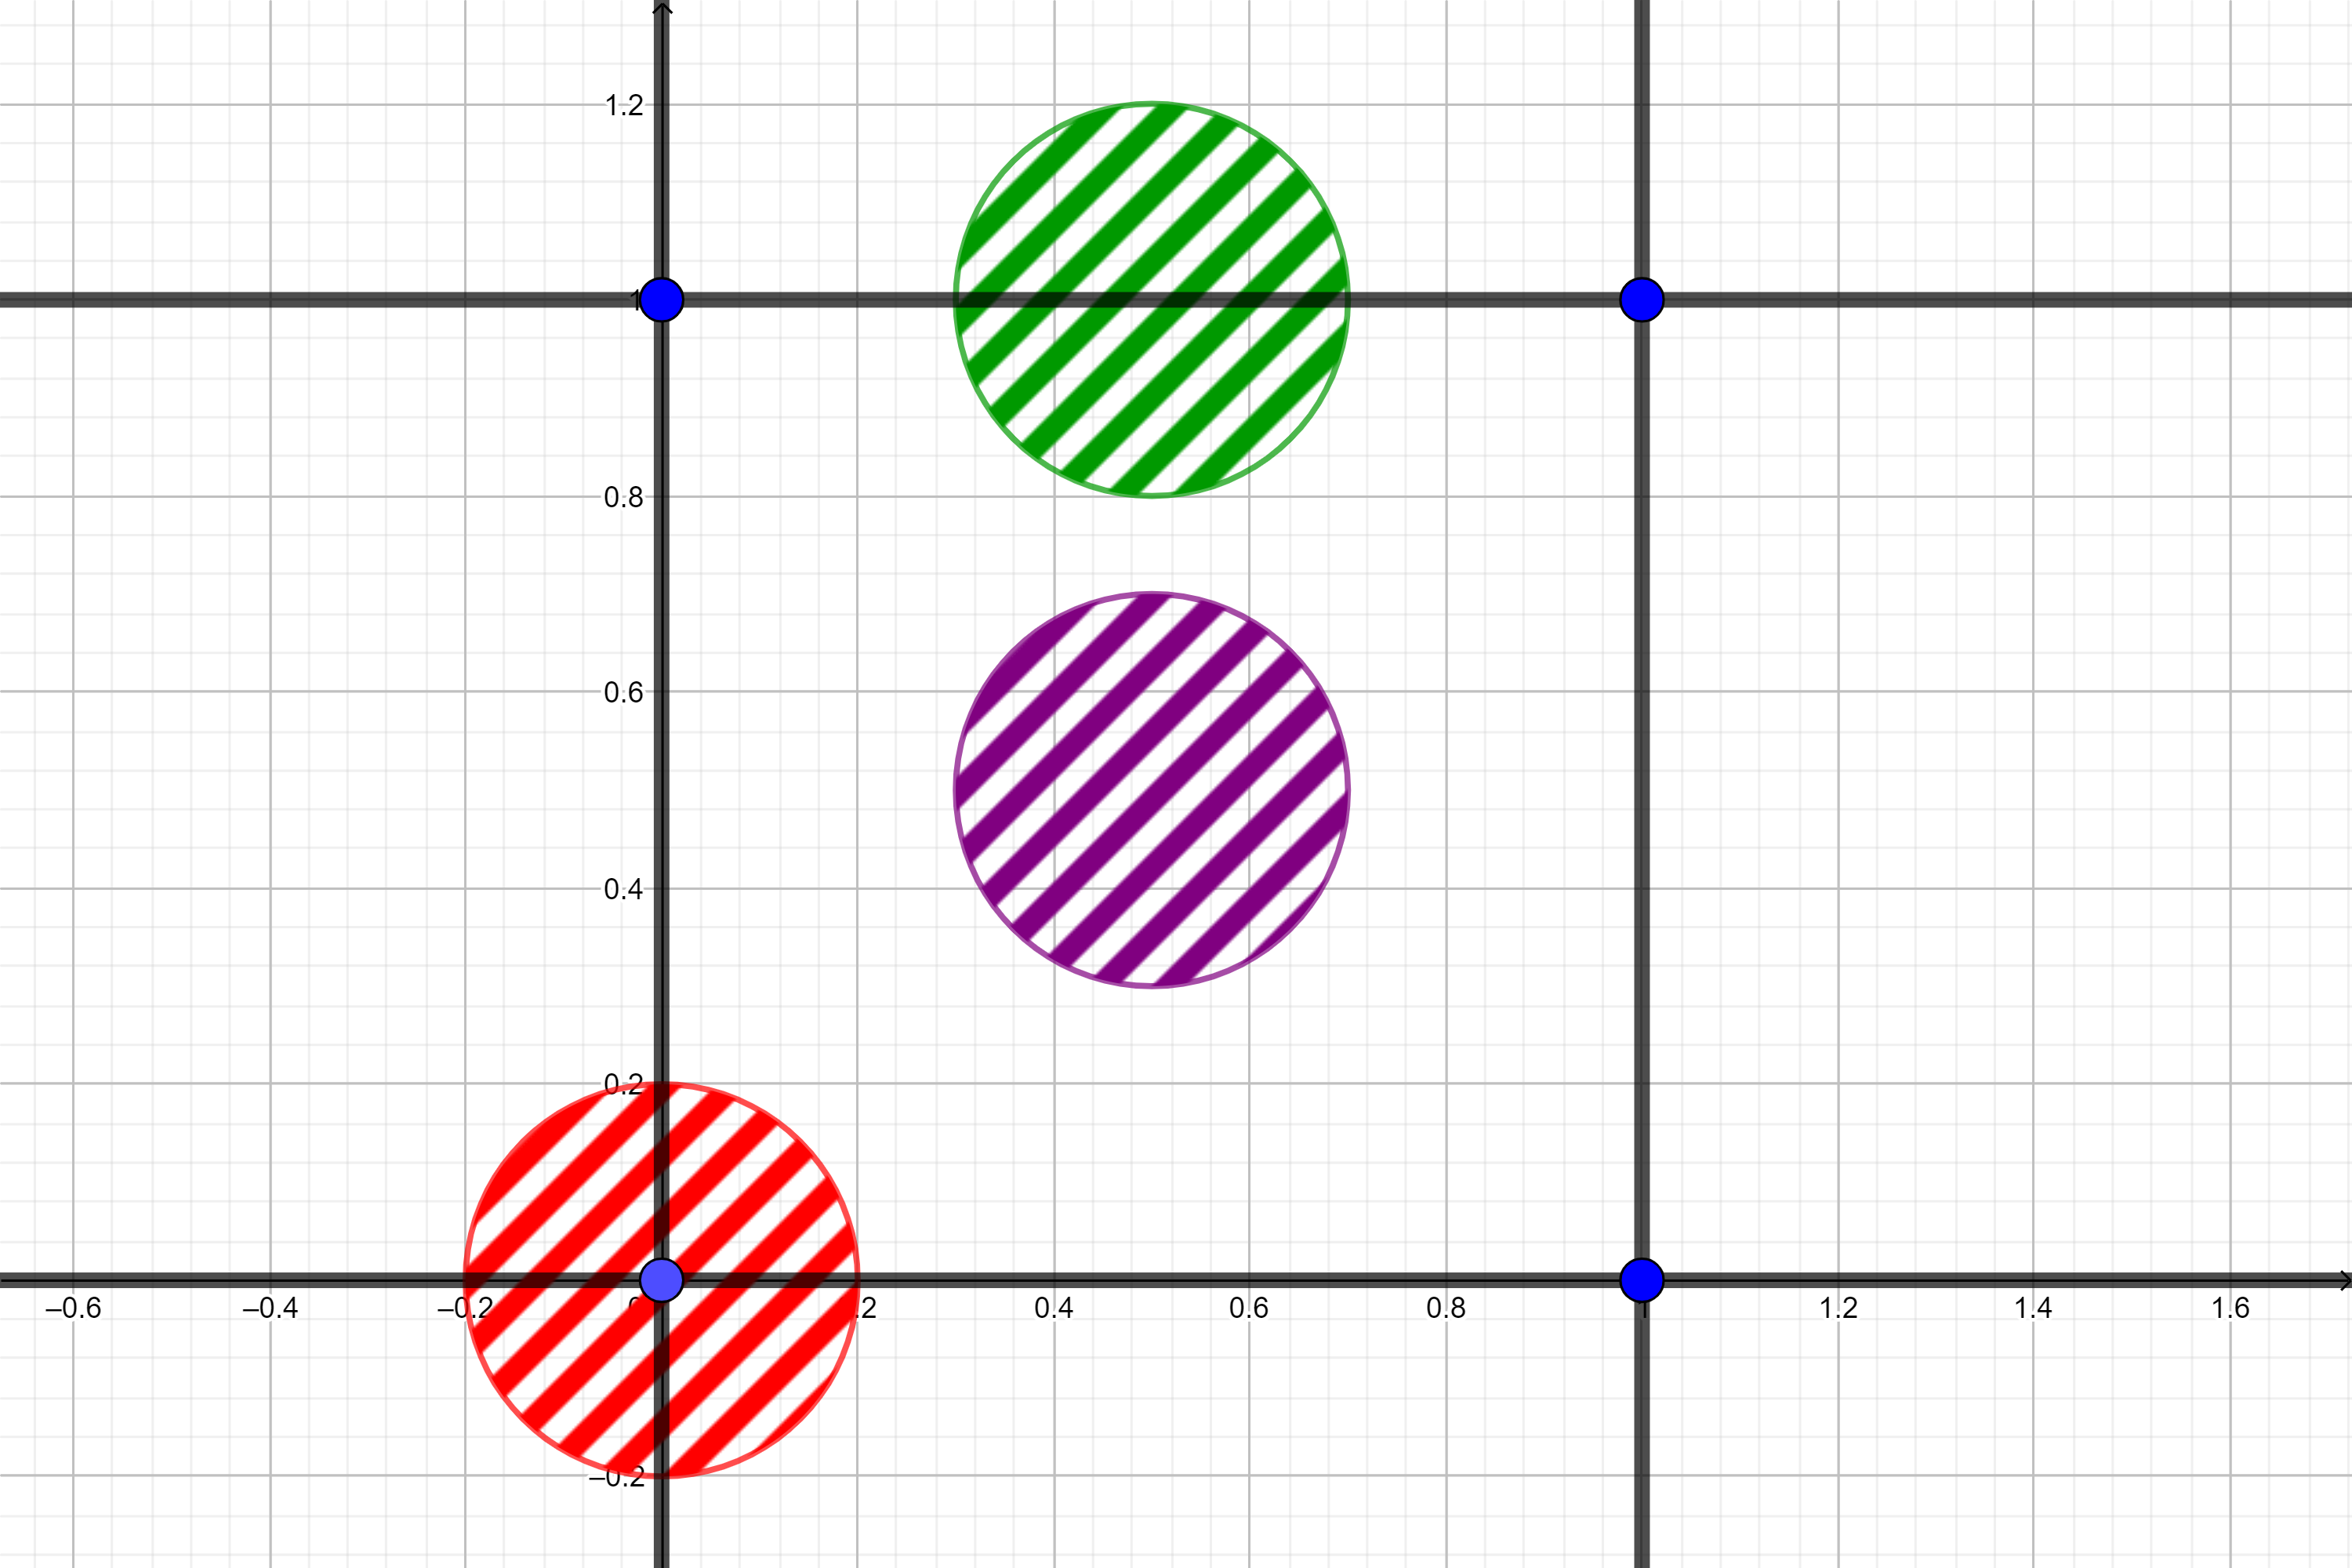
\includegraphics[width=5cm]{Reticle.png} 
\end{subfigure}
\begin{subfigure}{}
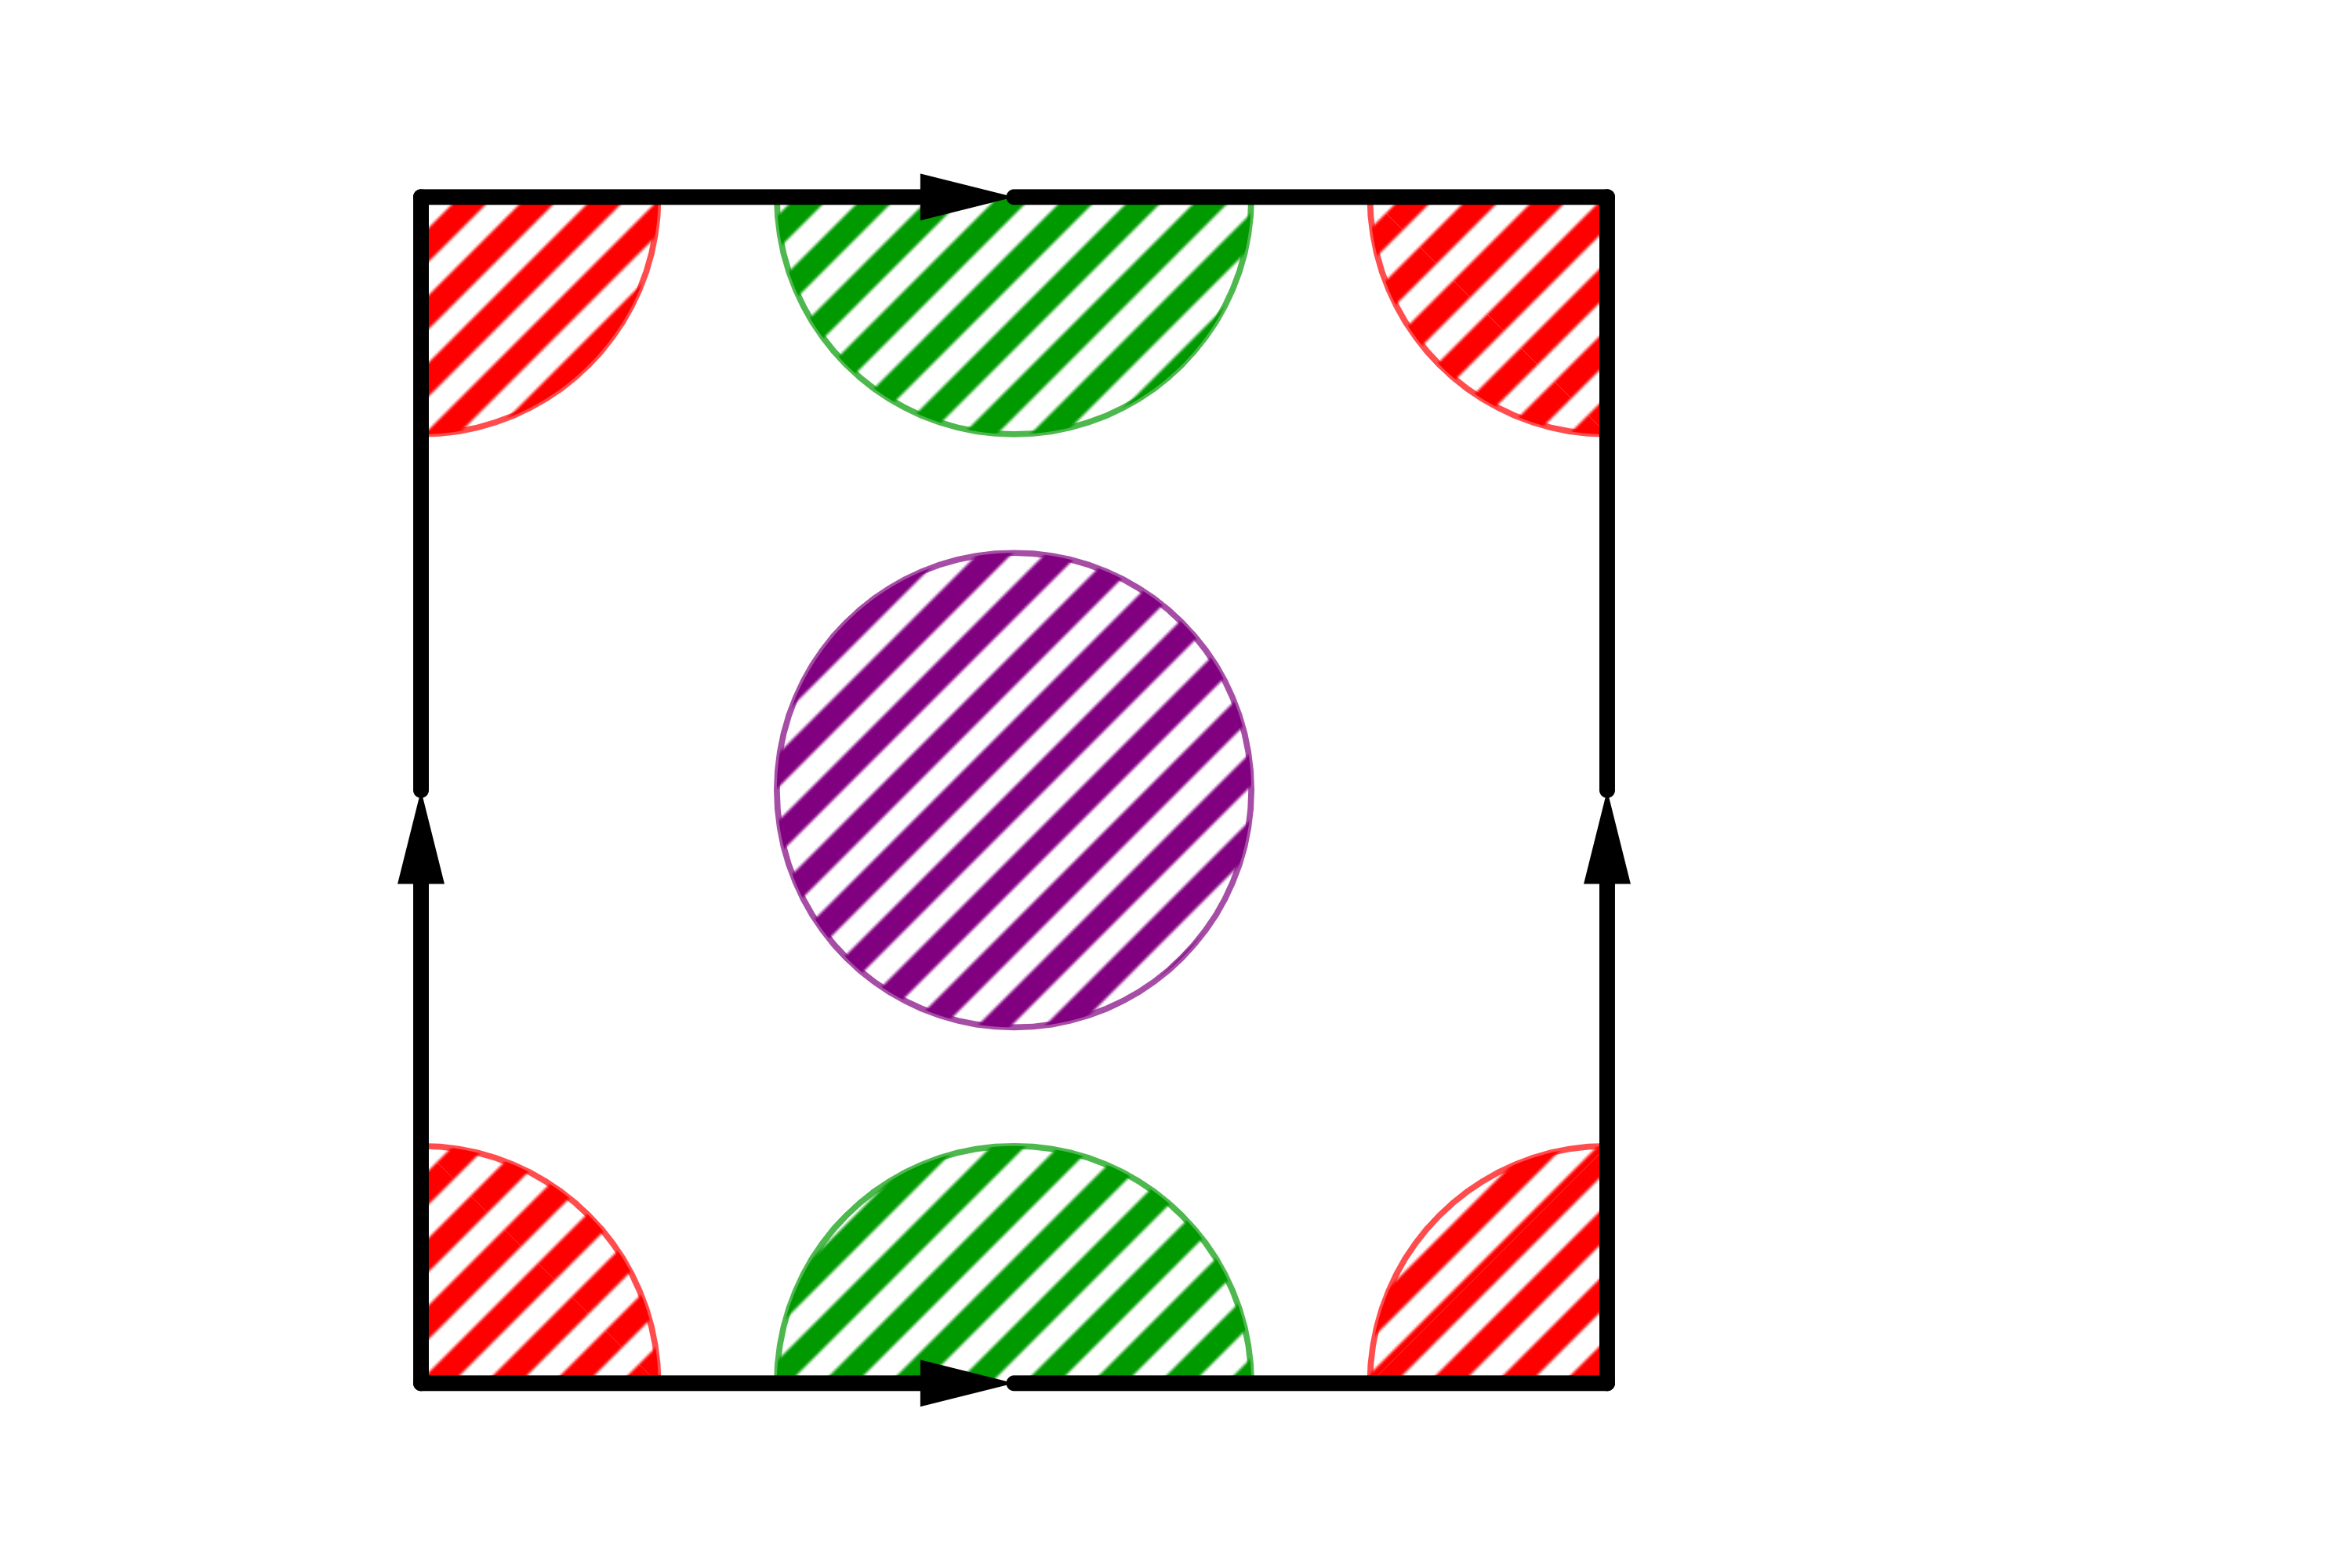
\includegraphics[width=5cm]{Quadrat.png} 
\end{subfigure}
\end{center}
\end{figure}
\end{frame}

\begin{frame}{Tors}
\begin{itemize}
\item Un reticle $\Gamma$ \'{e}s un grup de la forma $a\mathbb{Z}+b\mathbb{Z}$, on $a,b\in\mathbb{C}$ s\'{o}n tals que com a vectors de $\mathbb{R}^2$ s\'{o}n ortogonals.
\pause
\item Donats dos reticles $\Gamma_1=a_1\mathbb{Z}+b_1\mathbb{Z},\Gamma_2=a_2\mathbb{Z}+b_2\mathbb{Z}$, busquem un difeomorfisme o una aplicaci\'{o} biholomorfa (aplicaci\'{o} holomorfa bijectiva amb inversa holomorfa) que porti $\Gamma_1$ a $\Gamma_2$.
\pause
\item Ser\`{a} l'aplicaci\'{o} lineal que porti la base ortogonal $(a_1,b_1)$ a la base ortogonal $(a_2,b_2)$. Per tant sempre ser\`{a} un difeomorfisme de classe $C^{\infty}$. No obstant aix\`{o}, no sempre ser\`{a} holomorfa.
\pause
\item Nom\'{e}s ser\`{a} holomorfa quan la funci\'{o} sigui una dilataci\'{o}, una rotaci\'{o} o una reflexi\'{o}. De fet, existir\`{a} una funci\'{o} biholomorfa tal si i nom\'{e}s si
\[\frac{|b_1|}{|a_1|}=\frac{|b_2|}{|a_2|}.\]
\end{itemize}
\end{frame}

\begin{frame}{Teoria geom\`{e}trica d'invariants}
Per una banda considerem el conjunt de subconjunts de $\mathbb{C}^n$ que s\'{o}n zeros de polinomis. Per l'altra banda considerem el conjunt d'ideals de polinomis amb $n$ variables complexes.
\pause

A cada ideal $J\subseteq\mathbb{C}[z_1,\ldots,z_n]$ li podem fer correspondre el conjunt on s'anul\textperiodcentered len tots els seus polinomis
\[V(J)=\{(z_1,\ldots,z_n)\in\mathbb{C}^n\,|\,\forall f\in J\,\,f(z_1,\ldots,z_n)=0\}.\]
\pause

Tamb\'{e}, per cada $V\subseteq\mathbb{C}^n$ li podem fer correspondre l'ideal de polinomis que s'anul\textperiodcentered len sobre tots els punts de $V$
\[I(V)=\{f\in\mathbb{C}[z_1,\ldots,z_n]\,|\,\forall v\in V\,\,f(v)=0\}.\]
\pause

\emph{Nullstellensatz}: donat un ideal $J$ de polinomis, si hi apliquem aquests dos processos, obtenim
\[I(V(J))=\sqrt{J}=\{f\in\mathbb{C}[z_1,\ldots,z_n]\,|\,\exists n\in\mathbb{N}:f^n\in J\}.\]
\end{frame}

\begin{frame}{Teoria geom\`{e}trica d'invariants}
Donat un subconjunt algebraic $V\subseteq\mathbb{C}^n$, si $I$ \'{e}s el seu ideal de polinomis associat, constru\"{i}m l'anell quocient de funcions regulars $\mathbb{C}[z_1,\ldots,z_n]/I$. \'{E}s l'anell de les funcions que no es fan zero en $V$.
\pause

Llavors hi ha una aplicaci\'{o} anomenada espectre que permet recuperar el subconjunt algebraic a partir de l'anell de funcions $\mathbb{C}[z_1,\ldots,z_n]/I$. D'aquesta manera, els punts del subconjunt algebraic es corresponen amb ideals maximals de l'anell de funcions.
\end{frame}

\begin{frame}{Teoria geom\`{e}trica d'invariants}
Considerem l'acci\'{o} de $\mathbb{C}^*=\mathbb{C}\backslash\{0\}$ sobre $\mathbb{C}^2$ definida per
\begin{align*}
\mathbb{C}^*\times\mathbb{C}^2&\longrightarrow\mathbb{C}^2.\\
(t,(x,y))&\longmapsto(tx,t^{-1}y)
\end{align*}
\pause
Calculem el quocient de $\mathbb{C}^2$ per aquesta acci\'{o}: $\mathbb{C}^2/\sim$. Estudiem les \`{o}rbites.
\[[(x,y)]=\{(tx,t^{-1}y)\in\mathbb{C}^2\,|\,t\in\mathbb{C}^*\}=\{(x',y')\in\mathbb{C}^2\,|\,x'y'=xy\}\]
\pause
Per tant les \`{o}rbites s\'{o}n hip\`{e}rboles. L'\`{o}rbita de $(x,y)$, pot ser:
\begin{enumerate}
\item Si $x,y\neq0$, $[(x,y)]$ \'{e}s la hip\`{e}rbola $x'y'=xy$.
\pause
\item Si $x=0$, $y\neq0$, $[(0,y)]$ \'{e}s la recta complexa vertical $\{(0,y)\in\mathbb{C}^2\,|\,y\in\mathbb{C}^*\}$ sense l'origen.
\pause
\item Si $x\neq0$, $y=0$, $[(x,0)]$ \'{e}s la recta complexa horitzontal $\{(x,0)\in\mathbb{C}^2\,|\,x\in\mathbb{C}^*\}$ sense l'origen.
\pause
\item Si $x,y=0$, $[(0,0)]$ \'{e}s l'origen $\{(0,0)\}$.
\end{enumerate}
\end{frame}

\begin{frame}{Teoria geom\`{e}trica d'invariants}
\begin{figure}[ht!]
\begin{center}
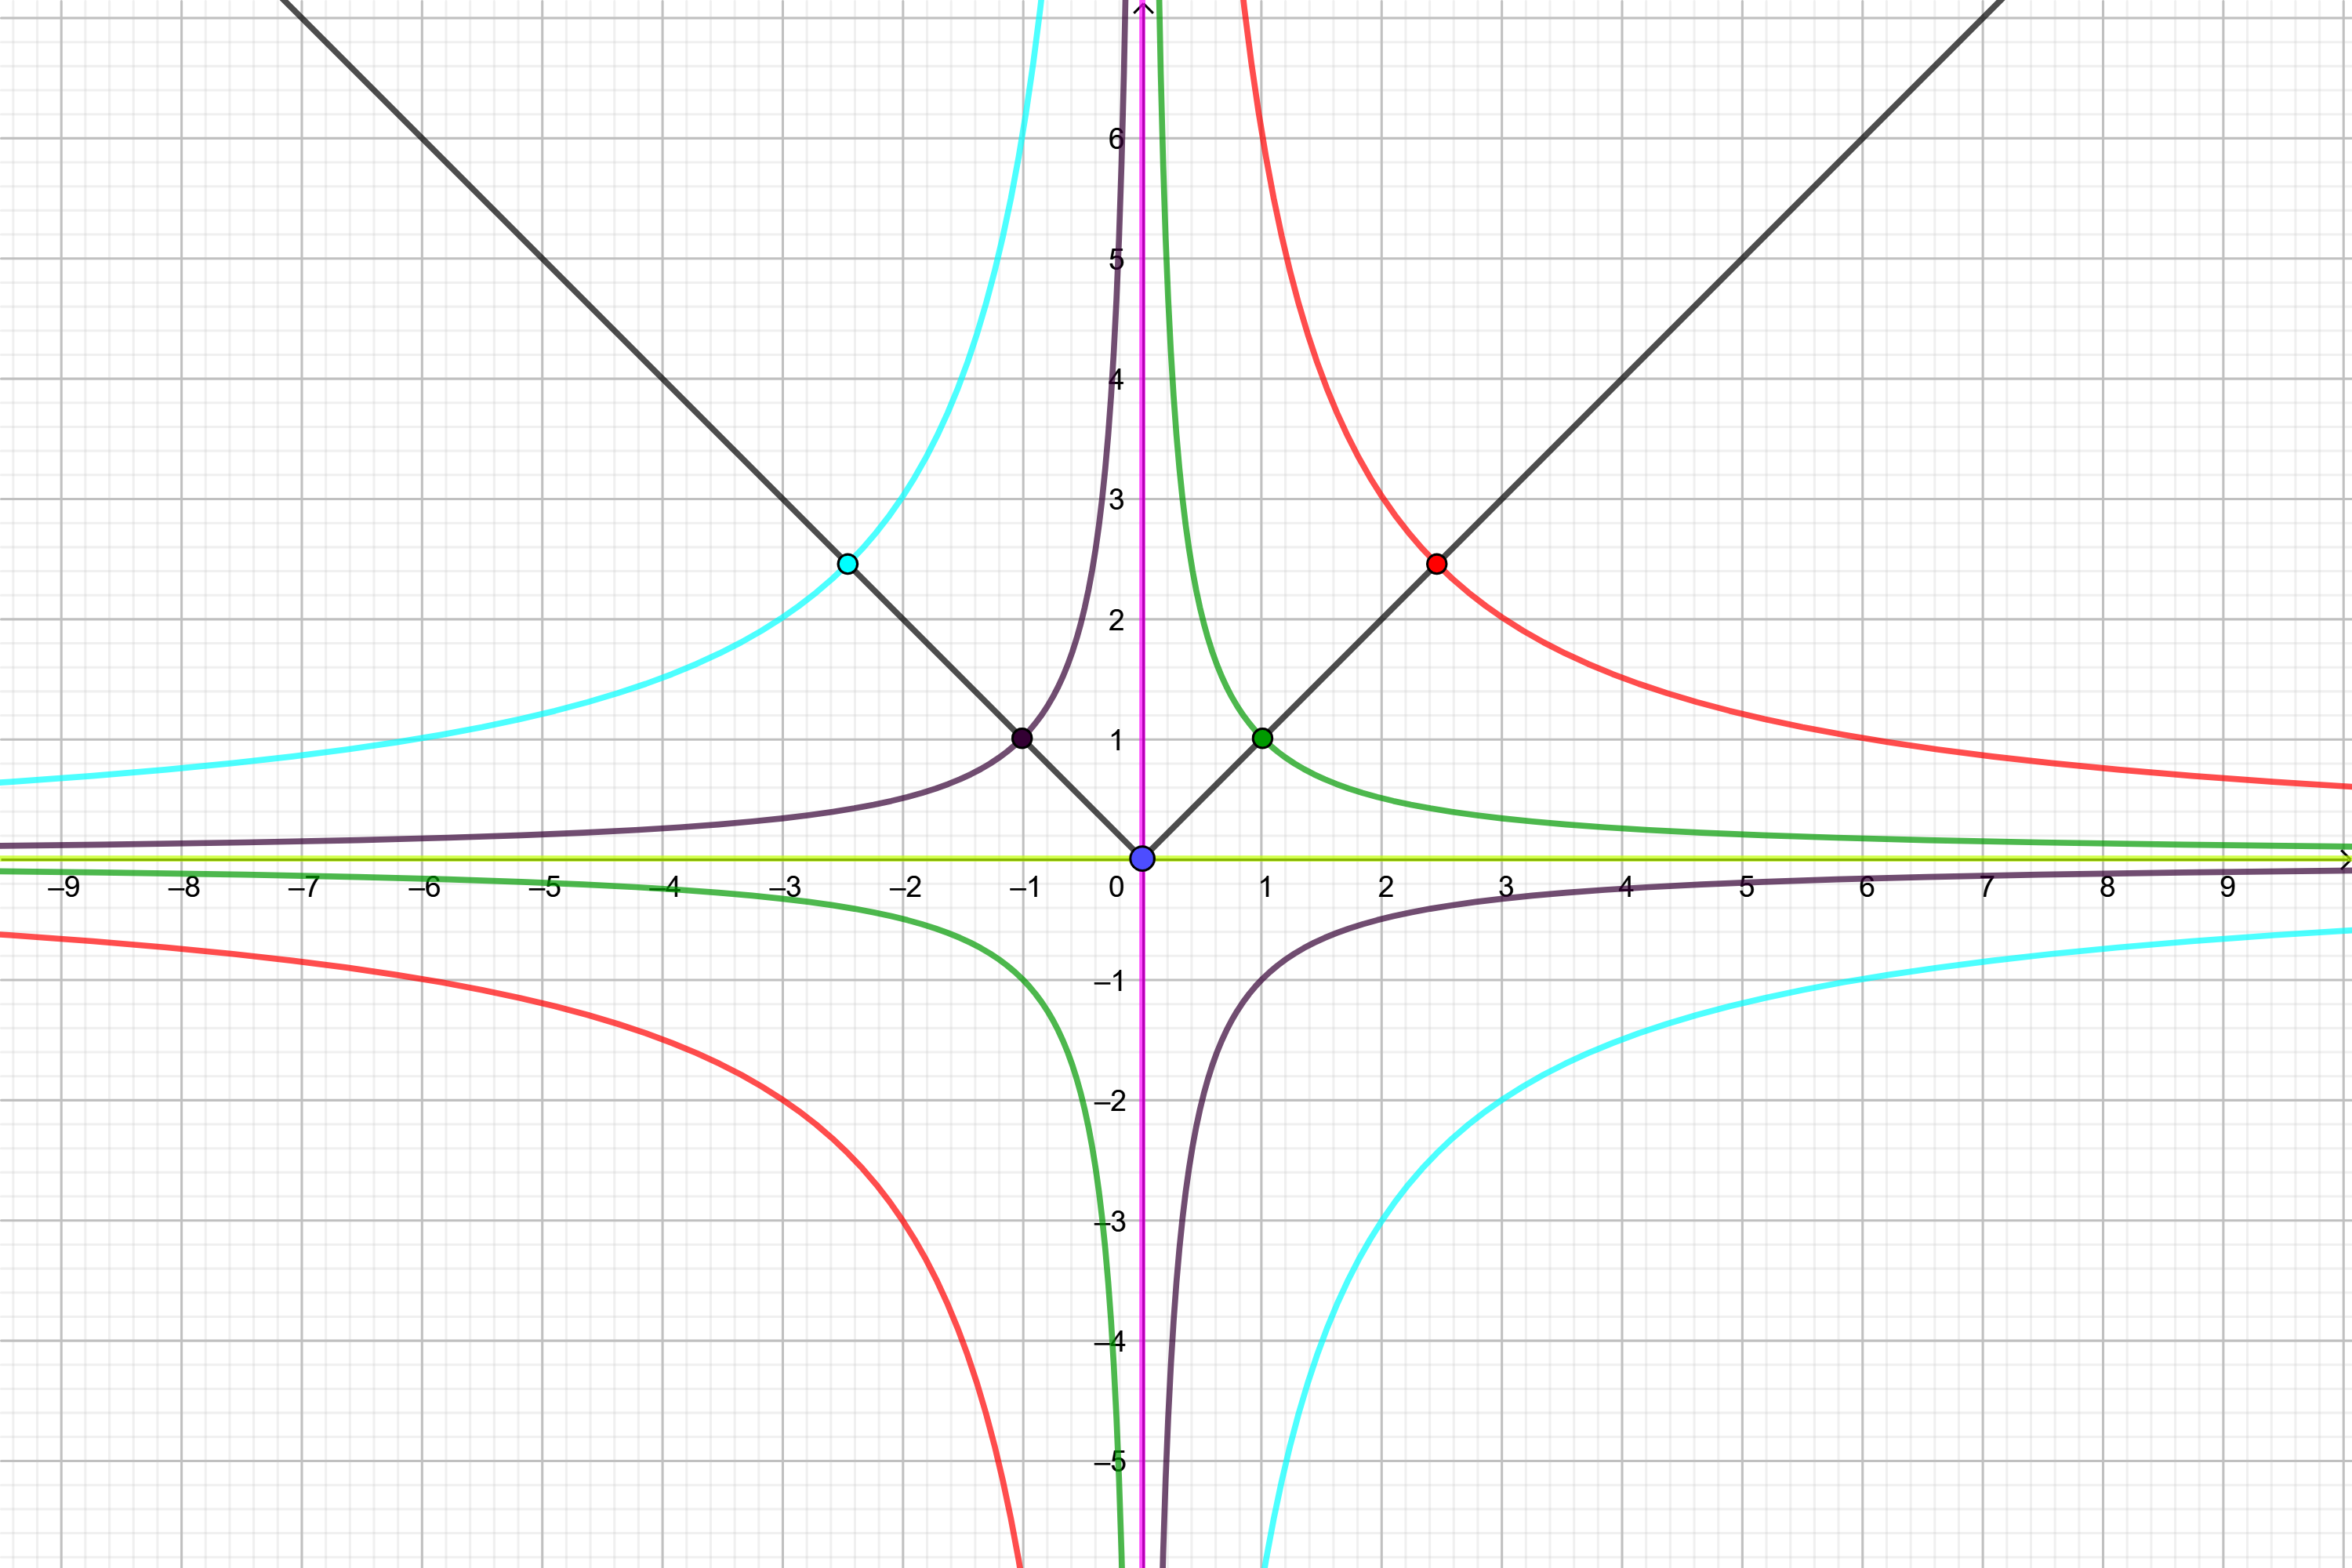
\includegraphics[width=8cm]{Hiperboles.png}
\end{center}
\end{figure}
\pause
Cada hip\`{e}rbola talla nom\'{e}s un cop la recta complexa negra. Per tant podem identificar $\mathbb{C}^2/\sim$ sense els eixos amb una recta complexa $\mathbb{C}$. Per tant, amb els eixos, $\mathbb{C}^2/\sim$ \'{e}s $\mathbb{C}$ amb tres or\'{i}gens. Aquest espai topol\`{o}gic no \'{e}s Hausdorff.
\end{frame}

\begin{frame}{Teoria geom\`{e}trica d'invariants}
Primer passem del conjunt algebraic $\mathbb{C}^2$ a l'anell de polinomis $\mathbb{C}[x,y]$. Sobre l'anell de polinomis, estudiem els ideals invariants per l'acci\'{o} de $\mathbb{C}^*$.
\pause
\[\mathbb{C}[x,y]^{\mathbb{C}^*}=\mathbb{C}[xy]\] Quan tornem aquest ideal $\mathbb{C}[xy]$ a un subconjunt algebraic per l'aplicaci\'{o} espectre, obtenim $\mathbb{C}$.
\pause

Hem obtingut un espai amb propietats molt m\'{e}s bones que el que hav\'{i}em obtingut fent directament el quocient, que era $\mathbb{C}$ amb tres or\'{i}gens.
\end{frame}
\end{document}
